
%The documentclass that we are going to we:
\documentclass[10pt,a4paper,fleqn]{article}
%\documentclass[10pt,a5paper,fleqn]{article}

\makeatletter
%%%To add dots in the section for the article class:
\renewcommand*\l@section{\@dottedtocline{1}{1.5em}{2.3em}}
%%%To remove the dots:
%\renewcommand\@dotsep{1000}
\makeatother

%%No longer required (from what I read on the internet, I might be mistaken).
%\usepackage[utf8]{inputenc}

%Packages for writing math:
\usepackage{amsmath}
\usepackage{amsfonts}
\usepackage{amssymb}

%Putting it simple, you need to put images.
\usepackage{graphicx}

%To write using more than on column.
\usepackage{multicol}
\usepackage{color}
\setlength{\columnseprule}{2pt}
\def\columnseprulecolor{\color{black}}
%\begin{multicols}{2}
%
%\end{multicols}

%To be able to use enumerate.
%\usepackage{enumerate}
\usepackage{enumitem}

%The caption package provides many ways to customise the captions in floating environments like figure and table, and cooperates with many other packages.
\usepackage{caption}

%The package also provides the H float modifier option of the obsolete here package. You can select this as automatic default with \floatplacement{figure}{H}. It is used to make sure that an image stays put where I want.
\usepackage{float}

%The hyperref package is used to handle cross-referencing commands in LATEX to produce hypertext links in the document. So that you can click on the text and it takes you to somewhere.
%So that I can click on the Contents section, and it takes me to the section I want:
\usepackage{hyperref}

%%\pagestyle{empty}
%%https://texfaq.org/FAQ-emptynum
%\parindent 0px

%%No page numbers:
%\usepackage{nopageno}

%In case, you don’t want the complete document to be indented, set the indentation length to zero with the command \setlength{\parindent}{0pt}.
%In the case where you want to indent a paragraph that is not indented, use the command \indent right above it. Please note that this command will only have an effect when \parindent is set to zero.
%\setlength\parindent{0pt}

%To change the border of our document. To change the geometry of our document.
\usepackage[left=2cm,right=2cm,top=2cm,bottom=2cm]{geometry}

%%To change the font we are going to be using. Number 1.
%% Choose one of the following fonts; obs.: use either XeLaTeX or LuaLaTeX
%\usepackage{fontspec}
%\setmainfont{YuKyokasho}
%\setmonofont{Hiragino Mincho ProN}
%\usepackage{fontspec}
%\setmainfont{Times New Roman}
%\setmonofont{Hiragino Mincho ProN}

%%To change the font we are going to be using. Number 2.
%% Choose one of the following fonts; obs.: use either XeLaTeX or LuaLaTeX
%\usepackage{xeCJK}
%\setCJKmainfont{YuKyokasho}
%\setCJKsansfont{Hiragino Mincho ProN}
%\setCJKmonofont{Hiragino Mincho ProN}

%%To put furigana when writing in Japanese.
%\usepackage{ruby}
%\renewcommand{\rubysep}{0.2ex}
%\ruby{学}{がく}
%\ruby{}{}

%tikzpicture
\usepackage{tikz}
\usepackage{scalerel}
\usepackage{pict2e}
\usepackage{tkz-euclide}
\usetikzlibrary{calc}
\usetikzlibrary{patterns, arrows.meta}
\usetikzlibrary{shadows}
\usetikzlibrary{external}
%\usepackage{circuitikz}

%pgfplots
\usepackage{pgfplots}
\pgfplotsset{compat=newest}
\usepgfplotslibrary{statistics}
\usepgfplotslibrary{fillbetween}

%colours
\usepackage{xcolor}

%% Font packages
%\usepackage[LGR,T1]{fontenc}
%\usepackage{lmodern}
%\usepackage{microtype}
%\usepackage{upgreek}
%\usepackage[misc]{ifsym}

% Maths and science packages
\usepackage{amsthm}
\usetikzlibrary{positioning}
\pgfplotsset{
		compat=1.16, % the version, it is good because even if there is an update, the graph won't change the look.
		samples=200, % the number of dots used to make the line.
		clip=false,
		my axis style/.style={%giving the name "my axis style"
			axis x line=middle,
			axis y line=middle,
			legend pos=outer north east,
			axis line style={
				->,
				very thick,
			},
			legend style={
				font=\footnotesize
			},
			label style={
				font=\footnotesize
			},
			tick label style={
				font=\footnotesize
			},
			xlabel style={
				at={
					(ticklabel* cs:1)
				},
				anchor=west,
				font=\footnotesize,
			},
			ylabel style={
				at={
					(ticklabel* cs:1)
				},
				anchor=west,
				font=\footnotesize,
			},
			xlabel=$x$,
			ylabel=$y$
		},
	}
	\tikzset{
		>=stealth
	}

%https://tex.stackexchange.com/questions/91201/change-the-appearance-of-grids-in-pgfplots
% grid style
\pgfplotsset{grid style={dashed,gray}}
%https://tex.stackexchange.com/questions/207212/how-do-i-change-the-font-size-of-the-axis-tick-labels-in-pgfplots
\pgfplotsset{every tick label/.append style={font=\footnotesize}}
%https://tex.stackexchange.com/questions/518926/tikz-opacity-of-colours
\usetikzlibrary{fadings}
\tikzfading
  [name = viesturs fading,
   inner color = transparent!0,
   outer color = transparent!100]

%https://tex.stackexchange.com/questions/435557/tikzpicture-horizontal-curly-brace
\usetikzlibrary{decorations.pathreplacing}

%https://tex.stackexchange.com/questions/614746/avoid-overlapping-of-the-vertical-line-of-arrow-and-path-label-in-tikz
\tikzset{
LM/.style = {very thin,
        {Bar[]Stealth}-%
        {Stealth[]Bar}
            },
% other common sty definitions like
every edge quotes/.append style= {font=\footnotesize}
        }

% Making the braket notation:
\newcommand{\bra}[1]{\left\langle #1 \right|}
\newcommand{\ket}[1]{\left| #1 \right\rangle}
\newcommand{\braketone}[2]{\left\langle #1 \middle| #2 \right\rangle}
\newcommand{\brakettwo}[3]{\left\langle #1 \middle| #2 \middle| #3 \right\rangle}

% So that I can name the section of the bibliography with whatever I want:
\usepackage{etoolbox}
\patchcmd{\thebibliography}{\section*{\refname}}{}{}{}

%%%%%%%%%%%%%%%%%%%%%%%%%

% The packages:

\usepackage{verbatim}

\usepackage{listings}

\usepackage{xcolor}

\usepackage[brazil]{babel} %*****

%%%%%%%%%%%%%%%%%%%%%%%%%

%%%%%%%%%%%%%%%%%%%%%%%%%

% Code styles and colours:

\definecolor{codegreen}{rgb}{0,0.6,0}
\definecolor{codegray}{rgb}{0.5,0.5,0.5}
\definecolor{codepurple}{rgb}{0.58,0,0.82}
\definecolor{electricpurple}{rgb}{0.75, 0.0, 1.0}
\definecolor{backcolour}{rgb}{0.96,0.96,0.96}
\definecolor{backbackcolour}{rgb}{0.96,0.96,0.96}
\definecolor{theshadowcolor}{rgb}{0.25,0.25,0.25}

\lstdefinestyle{mystyle}{
    backgroundcolor=\color{backcolour},
    commentstyle=\color{codegreen},
    keywordstyle=\color{magenta},
    numberstyle=\tiny\color{codegray},
%    stringstyle=\color{codepurple},
    stringstyle=\color{electricpurple},
    basicstyle=\ttfamily\footnotesize,
    breakatwhitespace=false,
    breaklines=true,
    captionpos=b,
    keepspaces=true,
    numbers=left,
    numbersep=10pt,
    showspaces=false,
    showstringspaces=false,
    showtabs=false,% mudar aqui para o Python
    tabsize=2,
    frame=shadowbox,
    frameround=ffff,
%    rulesepcolor=\color{blue},
%    rulesepcolor=\color{red},
%    rulesepcolor=\color{black},
    rulesepcolor=\color{theshadowcolor},
    showlines=true,
%    linewidth=0.5\linewidth,
%	extendedchars=true,
%	inputencoding=latin1,
	literate=
{á}{{\'a}}1
{à}{{\`a}}1
{ã}{{\~a}}1
{é}{{\'e}}1
{ê}{{\^e}}1
{í}{{\'i}}1
{ó}{{\'o}}1
{õ}{{\~o}}1
{ú}{{\'u}}1
{ü}{{\"u}}1
{ç}{{\c{c}}}1
}

%https://tex.stackexchange.com/questions/30512/how-to-insert-code-with-accents-with-listings

\lstset{style=mystyle}

%%%%%%%%%%%%%%%%%%%%%%%%%

\usepackage{forloop}
\usepackage{calc}

%%%%%%%%%%%%%%%%%%%%%%%%%

\usepackage[most]{tcolorbox}

\definecolor{mygray}{rgb}{0.5, 0.5, 0.5}

\definecolor{capri}{rgb}{0.0, 0.75, 1.0}

%%%%%%%%%%%%%%%%%%%%%%%%%


\author{Luigi Spreafico}
%\title{Programa de amigo oculto\\{\small (Versão 1)}}
\title{{\Huge Programa de amigo oculto}\\{\normalsize (Versão 1)}}
%\title{{\Huge Programa de amigo oculto}\\(Versão 1)}
\date{}

\begin{document}

\maketitle

\newpage

\tableofcontents

\newpage


\section{Linguagem de programação e seus módulos}

A linguagem utilizada é o Python\cite{Python}.
Os módulos utilizados são os seguintes:

\begin{lstlisting}[language=Python]
import numpy as np
\end{lstlisting}

O módulo do \texttt{numpy} \cite{NumPy} (normalmente utilizado como \texttt{np}) será utilizado para podermos embraralhar os nomes dos participantes.


\newpage


\section{Explicação do programa}

Aqui irei explicar o funcionamento do programa.
Para tal, primeiro irei apresentar um fluxograma.
Depois será feito uma explicação detalhada.
De qualquer forma, no próprio código tem vários comentários explicando a lógica por tráz do programa.

\subsection{Fluxograma}

\begin{figure}[H]
\centering
%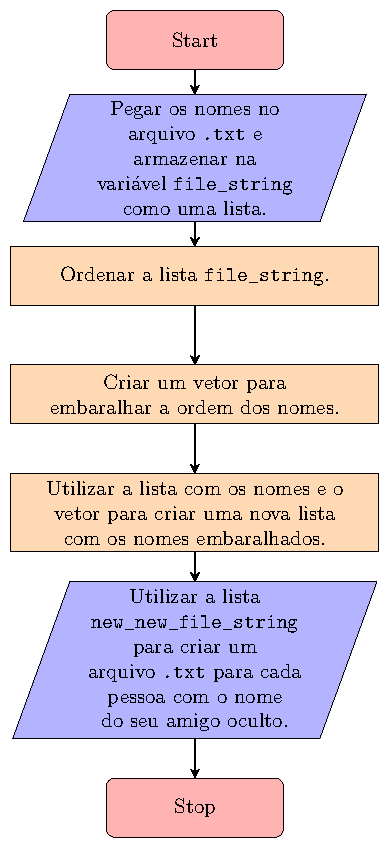
\includegraphics{00_7_imagem_1}
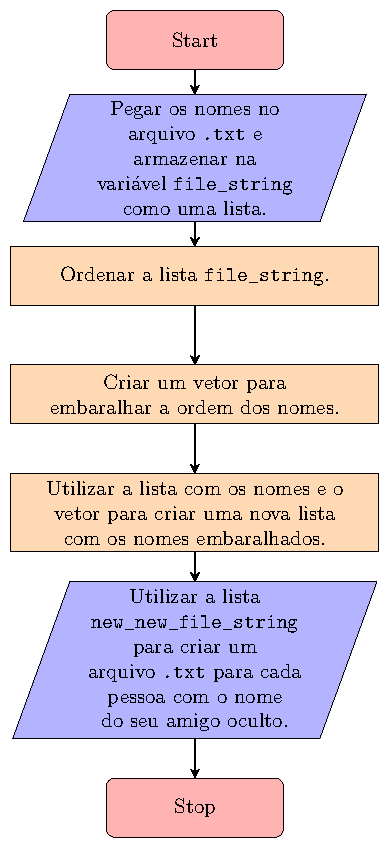
\includegraphics[scale=1.4]{00_7_imagem_1}
%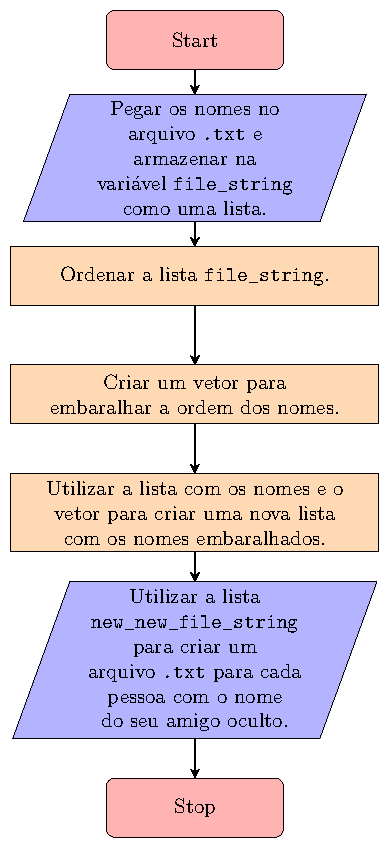
\includegraphics[width=.5\textwidth]{00_7_imagem_1}
\caption{Fluxograma do programa.}
\end{figure}

\newpage

\subsection{Explicação mais detalhada}

Aqui estarei explicando o programa.
Antes, quero dizer que existe mais de uma forma de se fazer as coisas que eu fiz, e que essa é a versão 1.
Além disso, que terá outras versões em que as coisas funcionarão de forma diferente.

No pedaço de código abaixo abrimos o arquivo \texttt{.txt} com os nomes das pessoas e armazenamos cada nome como um elemento de uma lista.
Utilizamos dessa forma porque se tivermos algum problema enquanto o arquivo está aberto ele vai fechar.
Tem outra forma de abrir um arquivo, mas que não fecha automaticamente, e com isso, dessa outra forma, acabamos tendo de lembrar de fechar o arquivo, além disso se tivermos algum problema enquanto o arquivo está aberto ele não vai fechar e podemos ter problemas quanto a isso.

\begin{lstlisting}[
				   language=Python,
				   caption={Pegando os nomes.},
				   numbers=none,
%				   title={Pegando os nomes.},
				   ]
with open('01_nome_das_pessoas_V1.txt') as f:
    file_string = f.readlines()
\end{lstlisting}

No pedaço de código abaixo pegamos a lista com os nomes e organizamos ela em orgem alfabetica.
Isso não é necessário.
Só coloquei pra testar a função.

\begin{lstlisting}[
				   language=Python,
				   caption={Ordenando os nomes.},
				   numbers=none,
%				   title={Ordenando os nomes.},
				   ]
file_string.sort()
\end{lstlisting}

No pedaço de código abaixo iremos criar um vetor que será utilizado para embaralhar a nossa lista de nomes.

\begin{lstlisting}[
				   language=Python,
				   caption={Criando um vetor para embaralhar.},
				   numbers=none,
%				   title={Criando um vetor para embaralhar.},
				   ]
idx = np.argsort(np.random.random(len(file_string)))
\end{lstlisting}

O pedaço de código acima funciona da seguinte forma:
\begin{enumerate}[label = \arabic*.]

\item \texttt{len(file\char`_string)}: pegamos o número de elementos da nossa lista

\item \texttt{np.random.random(len(file\char`_string))}: criamos um vetor com o mesmo número de elementos que o número de participantes. Onde este vetor é feito com números aleatórios de 0 até 1 (não incluindo o 1). Dessa forma, cada vez que rodarmos o programa iremos obter um vetor com elementos diferentes.

\item \texttt{np.argsort(np.random.random(len(file\char`_string)))}: Depois vamos e obtemos um vetor que nos diz a ordem dos indices de forma que esse nosso vetor fique em ordem correta.

\end{enumerate}
Abaixo temos um exemplo onde mostramos o que acontece passo a passo.

\begin{lstlisting}[
%				   language=Python,
				   caption={Exemplo criando um vetor para embaralhar no terminal do Python.},
				   numbers=none,
%				   title={Exemplo criando um vetor para embaralhar no terminal do Python.},
				   ]
>>> import numpy as np
>>> x = ['A', 'B', 'C', 'D', 'E']
>>> the_length = len(x)
>>> the_length
5
>>> the_random = np.random.random(the_length)
>>> the_random
array([0.39967192, 0.87469726, 0.14839865, 0.95127142, 0.44237115])
>>> idx = np.argsort(the_random)
>>> idx
array([2, 0, 4, 1, 3])
\end{lstlisting}

No pedaço de código abaixo criamos uma lista com o mesmo número de elementos que o número de participantes.

\begin{lstlisting}[
				   language=Python,
				   caption={Criando uma lista para os nomes embaralhados.},
				   numbers=none,
%				   title={Criando uma lista para os nomes embaralhados.},
				   ]
new_new_file_string = [0] * len(file_string)
\end{lstlisting}

No pedaço de código abaixo estamos utiliando o vetor com indices embaralhados \texttt{idx} para colocar de forma embaralhada os nomes na lista nova.

\begin{lstlisting}[
				   language=Python,
				   caption={Colocando os nomes na lista nova de forma embaralhada.},
				   numbers=none,
%				   title={Colocando os nomes na lista nova de forma embaralhada.},
				   ]
for i1 in range(len(new_new_file_string)):
    new_new_file_string[i1] = file_string[idx[i1]]
\end{lstlisting}

No pedaço de código abaixo pegamos e tiramos do final de cada nome o caracter \texttt{\symbol{92}n}.
Isso é importante para podermos gerar o nome dos arquivos.

\begin{lstlisting}[
				   language=Python,
				   caption={Retirando o caracter \texttt{\symbol{92}n}.},
				   numbers=none,
%				   title={Retirando o caracter \texttt{\symbol{92}n}.},
				   ]
for i1 in range(len(new_new_file_string)):
    new_new_file_string[i1] = new_new_file_string[i1].replace('\n', '')
\end{lstlisting}

No pedaço de código abaixo vamos criar um arquivo \texttt{.txt} para cada pessoa, e depois colocar dentro dele quem essa pessoa tirou.
A forma que vai ser criado o nome do \texttt{.txt} será para ser um amigo oculto de natal, para ser por exemplo de ano novo so mudar \texttt{\char`_natal\char`_AAAA} para \texttt{\char`_AnoNovo\char`_AAAA}.
E substituir \texttt{AAAA} pelo ano do amigo oculto (ou data completa: \texttt{DD\char`_MM\char`_AAAA}).

%# Aqui criar um arquivo .txt para cada pessoa, e depois colocar dentro dele quem essa pessoa tirou.
%# Obs.: a forma que vai ser criado o nome do .txt será para ser um amigo oculto de natal, 
%# para ser por exemplo de ano novo so mudar "_natal_AAAA" para "_AnoNovo_AAAA". 
%# E substituir AAAA pelo ano do amigo oculto (ou data completa: DD_MM_AAAA).

\begin{lstlisting}[
				   language=Python,
				   caption={Retirando o caracter \texttt{\symbol{92}n}.},
				   numbers=none,
%				   title={Retirando o caracter \texttt{\symbol{92}n}.},
				   ]
for i1 in range(len(new_new_file_string)):
    file_name = 'amigo_oculto_' + new_new_file_string[i1] + '_natal_2022' + '.txt'
    if ( i1 == ( len(new_new_file_string) - 1 ) ):
        the_length = len(new_new_file_string[0])
        with open(file_name, 'w') as f:
            f.write('O seu amigo oculto é: / A sua amiga oculta é:')
            f.write('\n')
            f.write('---> ')
            f.write(new_new_file_string[0])
            f.write('!'*(20-the_length))
            f.write('\n')
    else:
        with open(file_name, 'w') as f:
            the_length = len(new_new_file_string[i1+1])
            f.write('O seu amigo oculto é: / A sua amiga oculta é:')
            f.write('\n')
            f.write('---> ')
            f.write(new_new_file_string[i1+1])
            f.write('!'*(20-the_length))
            f.write('\n')
\end{lstlisting}

Agora mostrando graficamente como é feita a escolha.
Veja a figura abaixo (onde cada quadrado representa um elemento da lista final):

\begin{figure}[H]
\centering
%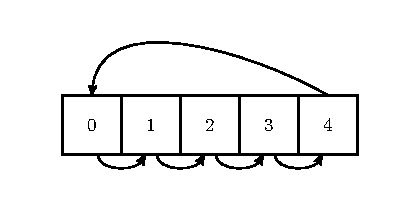
\includegraphics{00_7_imagem_2}
%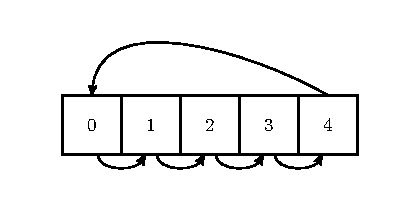
\includegraphics[scale=1.4]{00_7_imagem_2}
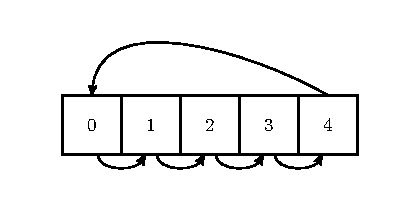
\includegraphics[width=.7\textwidth]{00_7_imagem_2}
\caption{Fluxograma do programa.}
\end{figure}

Na figura acima, podemos ver o quadrados representando um elemento da lista final (da lista embaralhada), onde os números representam os indices da lista e começamos pelo 0 por estarmos utilizando Python.
As setas mostram quem vai ter quem como amigo oculto, por exemplo, o nome que estiver no indice 1 terá a pessoa com nome no indice 2 como seu amigo oculto.




%\texttt{numpy}








\newpage


\section{Algumas observações}

Nesta versão é gerado um arquivo .txt para cada pessoa onde dentro tem o nome do seu amigo oculto ou da sua amiga oculta.
Teria de mandar para cada um o seu arquivo (por e-mail, whatsapp, ...).

\begin{tcolorbox}[
                 colback=white,
                 colframe=black,
                 sharp corners,
                 boxrule=2pt,
                 colbacktitle=white,
                 coltitle = black,
                 title=Exemplo de mensagem.]
Oi!

Tudo tranquilo?

No arquivo tem o nome do seu amigo oculto ou da sua amiga oculta, só abrir para ver.
\end{tcolorbox}

Nas próximas versões o objetivo é de por exemplo:
\begin{itemize}

\item Colocar algo para podermos inserir os nomes das pessoas, seja pelo terminal, ou por uma interfacie gráfica.

\item Colocar para enviar automaticamente para o e-mail das pessoas os resultados.

\item Quando for rodar o programa (no começo, antes de tudo) apargar todos os arquivos que nao sejam os necessários (por exemplo, se você for rodar uma segunda vez com menos pessoas, nessa versão ele já vai ter gerado algum arquivo \texttt{.txt} referente a uma pessoa que não vai participar e você teria de apagar manualmente).

\end{itemize}

Além disso, com esse código temos que só terá um círculo, por exemplo, tendo 5 pessoas teriamos $$1 \rightarrow 2 \rightarrow 3 \rightarrow 4 \rightarrow 5 \rightarrow 1$$ e nunca $$1 \rightarrow 2 \rightarrow 1$$ e $$3 \rightarrow 5 \rightarrow 4 \rightarrow 3$$, e, ninguém tira a si mesmo.

Outra observação a ser feita é que as exclamações no final de cada nome é para que todos os arquivos .txt tenham o mesmo número de caracteres,
de forma que todos os arquivos tenham o mesmo tamanho.
Isso porque como cada nome tem um número diferente de letras, acabariam tendo um arquivo com tamanho diferente.
Dessa forma, eu poderia acabar olhando sem querer que um arquivo é maior ou menor que o outro (mesmo sem abrir o arquivo)
e com isso ter uma dica de quem a pessoa tirou.
Dessa forma, eu não terei nenhuma dica sobre quem alguém tirou sem querer, e tudo pode ficar bem protegido.
A única forma de eu saber algo seria abrindo os arquivos gerados.

E por fim, no arquivo \texttt{01\char`_nome\char`_das\char`_pessoas\char`_V1.txt} colocar cada nome em um linha (como no exemplo).





















\newpage


\section{References}

\nocite{*}
%\bibliographystyle{plain}
\bibliographystyle{unsrt}
\bibliography{00_5_1_references}








\newpage


\section{O código}

%\lstinputlisting[language=Python]{01_amigo_oculto_V1.py}

\lstinputlisting[language=Python,
				 firstnumber=1,
				 firstline=1,
				 lastline=54]{01_amigo_oculto_V1.py}

\newpage

\lstinputlisting[language=Python,
				 firstnumber=55,
				 firstline=55,
				 lastline=111]{01_amigo_oculto_V1.py}




\end{document}











